\documentclass[../thesis.tex]{subfiles}

\begin{document}

\chapter{Experiments and Analysis}
In this chapter we will provide additional experimental results to validate the methods we proposed in Chapter 3 and demonstrate that our algorithm can be applied in a variety of settings -- not just satellite imagery. We will cover three data sets: CIFAR100, Stanford Dogs, and a newly developed data set consisting of posts from Reddit. In each of their sections, we will provide detailed descriptions of the data, the methods we employed, and the results.

\section{Experiment Set-up}
For each of the three data sets, we followed a standard experimental procedure. Similar to the FMOW data, the training data was bootstrapped $50$ and the classifier was fit to this data. This was done so that we could generate a distribution of estimator performance thereby allowing us to perform simple statistical tests. Moreover, we tested the algorithm proposed in Chapter 3 using both a k-nearest neighbors (KNN) classifier as well as a random forest (RF) classifier. We chose these two estimators because they have freely available implementations in the Scikit-learn machine learning framework as well as by testing with a variety of classifiers this enables us to validate that the results are not simply a unique quirk of a particular estimator, but rather a general property established by our methods. Since the feature extraction techniques had to specialized for each data set, we will discuss the methods we used when appropriate to provide context on how we transformed the data from its raw image or text form into something that a classifier, either flat or hierarchical, could use.

\section{CIFAR}

In this section I will describe the CIFAR data, and the experiments that we performed. The purpose of this first benchmark is to demonstrate how HCs, in general, can be used to get superior performance relative to a FC

\subsection{Data Description}
The CIFAR100 data set was developed in 2009 by Alex Krizhevsky in his 2009 paper, \textit{Learning Multiple Layers of Features from Tiny Images} \cite{krizhevsky2009learning}. The data consists of $60,000$ images scraped from the Internet from $100$ different labels. Additionally, the author hand-encoded $20$ groups of five labels (i.e., a meta-class however he calls them a ``super-class''). The full list of the labels and ``super-classes'' are provided in Appendix \ref{cifar100-labels}. Each of the classes have $600$ samples -- $500$ for training and $100$ for testing, and each image has been re-shaped to be $32 \times 32 \times 3$ pixels; the final channels corresponds to the red, green, and blue color channels because all of the images have color.

To extract features from the CIFAR100 image data, we employed the NASNet CNN model introduced in Chapter 2. Using this CNN yieled features vectors containing $4032$ dimensions \textbf{check if this is the correct number}. To visualize some of the label space to visualize how the CNN extracts features, we projected the original NASNet feature vector into two-dimensional space using principal component analysis (PCA). The result is shown in Figure \ref{fig:cifar-pca}.

\begin{figure}
    \centering
    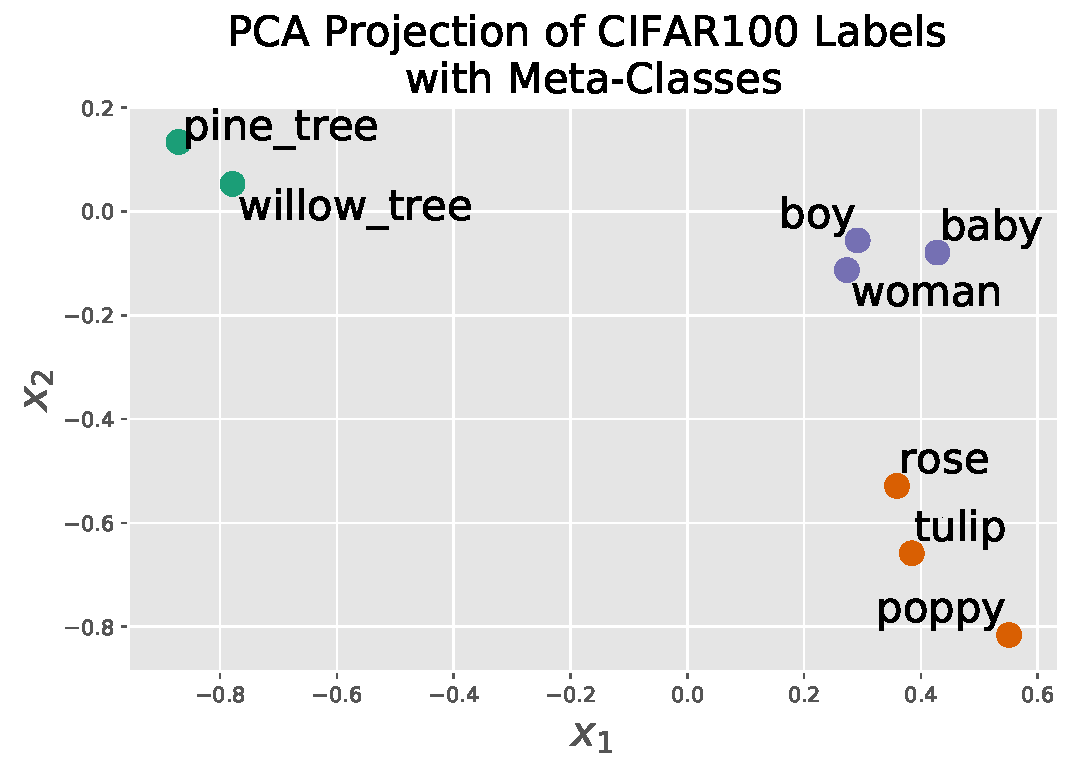
\includegraphics[width=\linewidth]{images/cifar-pca.pdf}
    \caption[CIFAR100 PCA Projection]{We randomly selected ten labels from the CIFAR100 data, generated its $\mathbf{V}$ matrix, and projected the original feature vector into two-dimensional space using PCA.}
    \label{fig:cifar-pca}
\end{figure}

While not perfect, it does seem that the CNN was able to encode meaningful relationships between the labels. For example, the animal labels -- the beaver, shark, and fox, are all close in their projected space to one another. Additionally, members of the household items ``super-class'': bottle and cup are also close to one another and far away from the rest of the classes.

\subsection{Experimental Results}
In this section I will describe the experimental results we got from the CIFAR data set. In particular we will highlight how employing a HC can lead to statistically significant improvements in estimator performance. As the graph will show, most the estimators are identical, so we cannot really distinguish between the methods, but by showing this data first we can demonstrate that indeed this method does make sense.

\section{Stanford Dogs}
In this section I will introduce the Stanford Dogs data set, discuss how it was developed, provide a bit context of places it has been employed in the past, and start to distinguish between our methods and other methodologies

\subsection{Data Description}
In this section, I will provide a description of the data, how it was it was developed, provide a breakdown of the labels that are contained in the data, and display some example images to contextualize how some of these classes are indeed quite similar to each other. 

\subsection{Experimental Results}
In this section, I will provide the experimental results from the Stanford dogs experiments. I plan to highlight our methods (such as the k-means based approached and community detection) can lead to statistically significant boosts in performance at the leaf level for different types of classifiers. I will also start to introduce some graphs to compare the time to train the classifiers so that we can explore trade-offs of employing certain techniques. For example, the LP-based approach does not seem to be on the efficient frontier when it comes to training time versus accuracy. 

\section{Reddit Data}
In this section, I will highlight how the Reddit data was developed, how we employed the techniques discussed in Chapter 2 to generate features for the text data. Afterwards I will again display the experimental results and provide some discussion to compare the various methods.

\subsection{Data Description}
In this section, I will describe Reddit for those who are unfamiliar with the website, detail how the data was created, and finally discuss how we parsed and generated features from the data. To make this real, I can potentially take one sample from the data, show how we got through the text pre-processing steps, and then finally project the data into a new space with features inferred from the spaCy model. One thought I have right now is to take that sample, get the vectors for all the words in the sample, use t-SNE to embed it into two dimensions, and then display that plot which shows how close or far away certain words are from one another. This might also be a good plot to use for our presentation. I like this idea; I'm going to do it because it helps nicely summarize what we are doing. We could also extend this for a few documents and try to show how certain sub-reddits we expect should be close and far away from one another. 

\subsection{Experimental Results}
This section will be quite similar to the previous ones; we're going to display the experimental results compare the various methods and explore the potential trade-offs the different hierarchical approaches.

\section{Conclusion}
In this section I will conclude by providing some general remarks that we can see from the three experimental data sets. In particular I will focus on comparing the various hierarchical methods, discussion how we were able to significantly outperform the flat classifier and also compare it to the standard spectral clustering based approach, and finally, discuss the computational trade-offs that exist when employing the various hierarchical methods. 

\end{document}